\documentclass[12pt]{article}
\usepackage[utf8]{inputenc}
\usepackage[T1]{fontenc}
\usepackage{graphicx}
\usepackage{xcolor}

%%novalidate

\usepackage{tikz}
\usepackage{calc}
\usepackage{booktabs}


% colors
\definecolor{color1}{HTML}{000060}
%\definecolor{color1}{HTML}{8C260F}
\definecolor{color2}{HTML}{333333}


% fonts
\usepackage{lmodern}
\renewcommand{\sfdefault}{lmss}
\renewcommand\familydefault{\sfdefault}
%%%


\usepackage{geometry}
\geometry{a4paper,
hmargin=20mm,vmargin=20mm,
head=0ex,foot=3ex}

\linespread{1.3}

\usepackage[hang]{caption}
\DeclareCaptionFormat{upper}{#1#2\uppercase{#3}\par}
\captionsetup{labelfont={bf,color=color2},textfont={normalsize,color=color2},format = upper,figurename=FIGURE,tablename=TABLE}

%%% fancy sections
\usepackage{titlesec}
%\titleformat{\chapter}{\sffamily\LARGE\bfseries\scshape\color{color1}}{\thechapter}{1em}{}[\titlerule]
\titleformat{\section}{\color{color1}\sffamily\Large\bfseries\uppercase}{\thesection}{1em}{}[\titlerule]
\titleformat{\subsection}{\color{color1}\sffamily\large\bfseries\uppercase}{\thesubsection}{1em}{}
\titleformat{\subsubsection}{\color{color1}\sffamily\bfseries\uppercase}{\thesubsubsection}{1em}{}
%%%

% head and foot
\usepackage{fancyhdr}
\pagestyle{fancy}
\lhead{}
\chead{}
\makeatletter
\rhead{\color{color2}\@date}
\makeatother
\newlength{\myheight}
\lfoot{
\settoheight{\myheight}{\thepage}
\raisebox{-2ex-0.5\myheight}{
\includegraphics[height=4ex]{images/logo}}
}
\cfoot{\color{color2}Cupboard: Requirements Specfication}
\rfoot{\color{color2}\thepage}
\renewcommand\headrulewidth{0pt}
\renewcommand\footrulewidth{0pt}

% custom titlepage
\makeatletter
\newcommand*\DefVar[1]{\@namedef{#1}##1{\global\@namedef{get#1}{##1}}}
\DefVar{summary}
\renewcommand{\maketitle}{
\begin{center}

\begin{tikzpicture}
    \node[draw=none,%color1,line width=0.4pt,
      fill=color1,
      inner sep = 10pt,
      text width=\textwidth-20pt,
      text centered
    ] {\color{white}\sffamily\bfseries\huge\@title};
\end{tikzpicture}
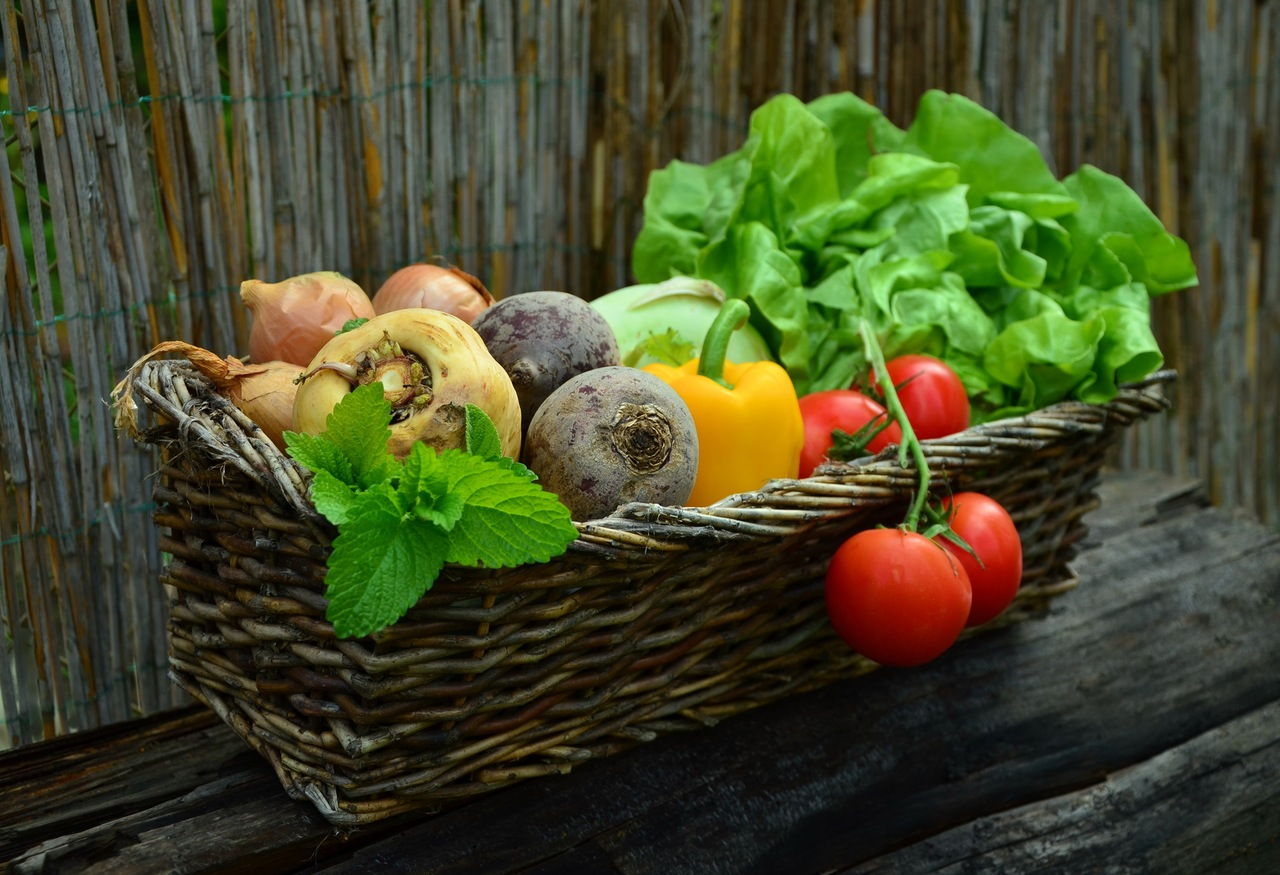
\includegraphics[width=\textwidth]{images/opening}\par
\sffamily\bfseries\Large\@author\par
\bigskip\medskip
{\color{color2}\normalfont\normalsize\textbf{Summary:}\\
\getsummary}
\end{center}
\clearpage
}
\makeatother
%%%

%%% fancy boxes
\usepackage{tcolorbox}
\usepackage{wrapfig}
\def\fullboxbegin{
\bigskip
\begin{tcolorbox}[colback=color1,colframe=color1,coltext=white,arc=0mm,boxrule=0pt]
}
\def\fullboxend{\end{tcolorbox}\medskip}
%
\def\leftboxbegin{
\begin{wrapfigure}{l}{0.5\textwidth}
\begin{tcolorbox}[colback=color1,colframe=color1,coltext=white,arc=0mm,boxrule=0pt]
}
\def\leftboxend{
\end{tcolorbox}
\end{wrapfigure}
}
%
\def\rightboxbegin{
\begin{wrapfigure}{r}{0.5\textwidth}
\begin{tcolorbox}[colback=color1,colframe=color1,coltext=white,arc=0mm,boxrule=0pt]
}
\def\rightboxend{
\end{tcolorbox}
\end{wrapfigure}
}
%
\newcounter{frames}
\def\frameboxbegin#1{
\bigskip
\refstepcounter{frames}
\begin{tcolorbox}[colback=white,colframe=color1,arc=0mm,title={\MakeUppercase{\textbf{Frame \arabic{frames}}: #1}}]
}
\def\frameboxend{
\end{tcolorbox}
}
%%%

%custom Requirements titles
\usepackage{titlesec}
%\usepackage{hyperref}
%Funtional
\titleclass{\requirement}{straight}[\subsubsection]
\newcounter{requirement}
\titleformat{\requirement}
  {\color{color1}\sffamily\bfseries}{}{0em}
  {\refstepcounter{requirement}FR \therequirement:~}
\titlespacing*{\requirement}{0pt}{3.25ex plus 1ex minus .2ex}{1.5ex plus .2ex}

\setcounter{tocdepth}{4}
\makeatletter
  \def\toclevel@requirement{5}
  \def\l@requirement{\@dottedtocline{5}{3.8em}{3.2em}}
\makeatother
%%%


%requirements table enviromnent
\newenvironment{reqtable}
{
    \medskip
    \begin{tabular}{|p{3.5cm}|p{11cm}|}
    \hline
}
{\end{tabular}}


\usepackage{lipsum}

%%%%%%%%%%%%%%%
% Title Page
\title{Cupboard:\\Requirements Specfication}
\author{Team 8:\\Clare Doran, Abdul Ghani, Ucizi Mafeni, Luke Needham, Soumya Singh}
\date{\today}
\summary{
A web app built with the intention of helping reduce food waste
}
%%%%%%%%%%%%%%%

\begin{document}
\maketitle

\tableofcontents
\clearpage
%glossary
%define "active" listing
%define listing
%define immutable
%define trade
\section{Introduction}
7 million tonnes of food goes to waste in the UK, more than half of which is 
edible (https://www.lovefoodhatewaste.com/node/2472).
Meanwhile,  many people throughout the country struggle to put together enough 
money for food, with food banks becoming busier every year
(https://www.trusselltrust.org/2015/11/18/uk-foodbank-use-still-at-record-levels-as-hunger-remains-major-concern-for-low-income-families/)

Cupboard aims to be a system that allows users to painlessly find and share food
that would otherwise go to waste. It should be quick and easy to use as it is
too easy to just throw away food. 
It will also allow users to arrange collection in a manner that does not force
them to disclose their house address or any other details they wish to keep
private.


\section{Project Scope}
Cupboard will facilitate the sharing of food between users. It will do so in a
manner that is as simple as possible, as we want to discourage people from
taking the easy route of simply binning food they wont eat.
There will be a simple points-based system and a ranking system in order to
encourage sharing of food and reassure other users that the quality of food is
likely to be good. When some food has been ‘successfully exchanged’ both
parties will get points and will be able to rate each other. If users wish to
participate, there will be a simple public leaderboard.
Users can set their dietary requirements (allergies, religious etc.) and have
results automatically filtered. 
There will be a messaging system (in order to arrange collection) and a comments
system (in order to view interest in the item and ask questions).


\section{Domain Analysis}
There are a couple of examples of food sharing sites/apps such as:
\begin{itemize}
    \item foodsharing.de(https://foodsharing.de/): A German food sharing site
        that allows users (just like our site) to trade food that is going out
        of date with other users to reduce food waste.
        However it is only available in Germany.
    \item Olio (https://olioex.com/): Mobile app with strong UK presence.
        A key distinguishing feature is "Drop Boxes".
        These are local stores/cafes where users can drop off food they'd like
        to be shared.
    \item SharingFood
        (https://itunes.apple.com/us/app/sharing-food/id992111062?mt=8):
        Mobile app based in Italy.
        Seems to be fairly new and so has a very small user base.
\end{itemize}


\section{Proposed Deliverables}
(Gantt Chart Goes here)

\section{Identified, Risks, Assumptions, Dependencies and Constraints}
\begin{itemize}
    \item User Location: How much information about the user's location can we
        make publicly available without putting their security ar risk?
    \item Assuming google maps should be able to find the addresses entered by
        the user.The location functionality is completely dependent on the
        Google Maps API.
\end{itemize}

\section{Solution Requirements}
\subsection{Functional Requirements}
%move section of speech to development approach
N.B. Due to the highly time-sensitive nature of the project, any low priority
requirements (and thier linked dependencies) may not be implemented.
As such, all low priority requirements are inherently unessential to the
system, and it will remain fully operational with or without them.

\requirement{"About Us" page}
\label{fr:about-us}

\begin{reqtable}
    Description        & All users should have access to a page that contains 
                        information about the web app. This includes:
                        
                        \begin{itemize}
                            \itemsep-1em
                            \item A short description about the purpose of the
                                app.
                            \item Contact information
                            \item Terms and Conditions of use
                            \end{itemize}
                        \\
    \hline
    Priority           & Medium\\
    \hline
    Dependencies       & None\\
    \hline
    Expected results   & User able to access the page.
                        
                        Page contains all the information stated in the
                        description.\\
    \hline
    Exception Handling & \\
    \hline
\end{reqtable}


\requirement{Error-Reporting System}
\label{fr:error-reporting}

\begin{reqtable}
    Description        & Users should be able to report any errors they notice
                        to the webmaster.
                        Each error report should have:

                        \begin{itemize}
                            \itemsep-1em
                            \item A title, which is a brief description of the
                                error (max. 50 chars)
                            \item A more detailed description of the error
                                (max. 500 chars)
                        \end{itemize}
                        \\
    \hline
    Priority           & Medium\\
    \hline
    Dependencies       & \autoref{fr:about-us}\\
    \hline
    Expected results   & User can successfully send error report\\
    \hline
    Exception Handling & 
                        \begin{description}
                            \itemsep0em
                            \item [User cannot send error report:] use email on
                                "About us" page to contact webmaster
                        \end{description}
                        \\
    \hline
\end{reqtable}


\requirement{User Feedback System}
\label{fr:user-feedback}

\begin{reqtable}
    Description        & Users should be able to provide feedback regarding
                        their experience using the web app to the webmaster.
                        This should be done in the form of a feedback form,
                        which should have the following fields:

                        \begin{itemize}
                            \itemsep-1em
                            \item A title, which is a brief description of the
                                feedback report(max. 50 chars)
                            \item The main feedback report (max. 1000 chars)
                        \end{itemize}
                        \\


    \hline
    Priority           & Low\\
    \hline
    Dependencies       & \autoref{fr:error-reporting} (Error Reporting)\\
    \hline
    Expected results   & User's can successfully send feedback report\\
    \hline
    Exception Handling & 
                        
                        \begin{description}
                            \itemsep0em
                            \item [User unable to send feedback form]: report 
                                error to webmaster
                        \end{description}
                        \\
    \hline
\end{reqtable}


\requirement{User sign up}
\label{fr:user-sign-up}

\begin{reqtable}
    Description        & The User should be able to create an account by 
                        following the registration process.

                        Registration will involve:

                        \begin{itemize}
                            \itemsep-1em
                            \item Getting the user registration details
                                (see \autoref{fr:registration-details}).
                            \item Getting the user to accept that they are at 
                                least 18 years old.
                            \item Getting the user to agree to the Terms and
                                Conditions of use (see \autoref{fr:about-us}).
                        \end{itemize}
                        \\
    \hline
    Priority           & High\\
    \hline
    Dependencies       & \autoref{fr:error-reporting},
    \autoref{fr:registration-details} (Get user registration details),
    \autoref{fr:about-us} (About us page)
                        \\
    \hline
    Expected results   & Following account creation, the user will be able to 
                        login using their provided username and password\\
    \hline
    Exception Handling & 
                        
                        \begin{description}
                            \itemsep0em
                            \item [User unable to create account:] report error
                                to webmaster
                        \end{description}
                        \\
    \hline
\end{reqtable}

\requirement{Get User Registration Details}
\label{fr:registration-details}

\begin{reqtable}
    Description        & During sign-up, the user should provide the following
                        details in order to successfully complete the sign-up
                        process:

                        \begin{itemize}
                            \itemsep-1em
                            \item username (must be unique)
                            \item email address
                            \item password
                            \item physical address
                            \item post code (must be valid)
                        \end{itemize}
                        
                        In addition, the user should also be given the option
                        to fill in their Dietary Requirements and Allergy 
                        Information. However, it is not mandatory to fill in 
                        these details in order to complete registration.

                        \\
    \hline
    Priority           & High\\
    \hline
    Dependencies       & \autoref{fr:error-reporting},
    \autoref{fr:validation} (Validate User Details), 
    \autoref{fr:dietary-requirements} (Dietary Requirements), 
    \autoref{fr:allergy-information} (Allergy Information)\\
    \hline
    Expected results   & User inputs all valid fields and proceeds to complete
                        registration\\
    \hline
    Exception Handling & 
                        
                        \begin{description}
                            \itemsep0em
                            \item [User unable to fill in registration details:]
                                report error to webmaster
                            \item [User inputs invalid details:] should be
                                validated as described in \autoref{fr:validation}
                        \end{description}
                        \\
    \hline
\end{reqtable}

\requirement{Validate Registration Details}
\label{fr:validation}

\begin{reqtable}
    Description        & Information in the registration form should be
                        validated as follows:
                        
                        username: checked against database to see if its unique

                        email-address: adheres to general email structure 
                        (<someuser>@<somehost>.<com/net\ldots>)

                        password: minimum length of 7 characters, alphanumeric,
                        contains one symbol from valid symbol list
                        (refer to glossary)

                        postcode: is actual valid postcode 
                        (check in UK postcode directory)

                        If there exists an invalid input on submission,
                        the form must be rejected and the user must be
                        notified of their error
                        (i.e highlight incorrect field and place error message
                        next to it)
                        \\
    \hline
    Priority           & High\\
    \hline
    Dependencies       & \autoref{fr:error-reporting}\\
    \hline
    Expected results   & Validation system correctly highlights any invalid
                        fields\\
    \hline
    Exception Handling & 
                        
                        \begin{description}
                            \itemsep0em
                            \item [Validation system doesn't meet specified 
                                requirements:]
                                report error to webmaster
                        \end{description}
                        \\
    \hline
\end{reqtable}

\requirement{Account Activation}
\label{fr:activation}

\begin{reqtable}
    Description        & 
                        Once the user has provided the registration details,
                        an email with an account activation link
                        should be sent to the provided email address. The user
                        should then be able to follow the activation link in
                        order to activate their account.\\
    \hline
    Priority           & Low \\
    \hline
    Dependencies       & \autoref{fr:error-reporting}\\
    \hline
    Expected results   & After the user follows the activation link,
                        they should be able to login to their account using
                        the login details they provided during registration\\
    \hline
    Exception Handling & 
                        \begin{description}
                            \itemsep0em
                            \item [Incorrect email address provided:]
                                the user should have the
                                option to correct the provided email address.
                            \item [Activation link doesn't work:] the user
                                should have the option to request another
                                activation link.
                            \item [Activation system doesn't work:] report
                                error to webmaster
                        \end{description}
                        \\
    \hline
\end{reqtable}

\requirement{Password Reset Facility}
\label{fr:password-reset}

\begin{reqtable}
    Description        & If a registered user forgets their password, they
                        should be able to request a password reset link.
                        
                        They should provide a valid email address within
                        the request. If the provided email address is linked
                        to an account on the system, a password reset link
                        should be sent to that email.

                        Upon following the password reset link, the user should
                        be able to set a new password.
                        \\
    \hline
    Priority           & Low\\
    \hline
    Dependencies       & \autoref{fr:validation}\\
    \hline
    Expected results   & User able to successfully reset password\\
    \hline
    Exception Handling & 
                        
                        \begin{description}
                            \itemsep0em
                            \item [User unable to reset password:] report error
                                to webmaster.
                            \item [Email doesn't meet validation
                                standards set in \autoref{fr:validation}:]
                                Prevent submission of password reset request.
                                Notify user that invalid email was entered.
                        \end{description}
                        \\
    \hline
\end{reqtable}


\requirement{User Dashboard}
\label{fr:user-dashboard}

\begin{reqtable}
    Description        & Following login, all registered users should have
                        access to a personal
                        dashboard where they can do the following:
                        
                        \begin{itemize}
                            \itemsep-1em
                            \item edit their personal details
                            \item edit their current dietary requirements
                            \item edit their allergy information
                            \item view their user score and rating
                        \end{itemize}

                        \\
    \hline
    Priority           & High\\
    \hline
    Dependencies       & \autoref{fr:edit-profile} (Edit Profile),
    \autoref{fr:dietary-requirements},
    \autoref{fr:allergy-information},
    \autoref{fr:user-score} (User Score),
    \autoref{fr:user-ratings} (User Rating)
    \\
    \hline
    Expected results   & User is able to access and edit all personal
                        information from the dashboard\\
    \hline
    Exception Handling & 
                        \begin{description}
                            \itemsep0em
                            \item [Registered and logged-in user can't access
                                dashboard:] notify webmaster of error
                        \end{description}
                        \\
    \hline
\end{reqtable}


\requirement{Edit Profile}
\label{fr:edit-profile}

\begin{reqtable}
    Description        & A user should be able to change their personal details
                        this includes:

                        \begin{itemize}
                            \itemsep-1em
                            \item their username
                            \item their email address
                            \item their password
                            \item their dietary requirements
                            \item their allergy information
                        \end{itemize}

                        All changes to personal details will be validated under
                        the standards mentioned in
                        \autoref{fr:validation}.

                        With regards to dietary requirements and allergy
                        information, users will be able to select whichever
                        categories listed in \autoref{fr:dietary-requirements}
                        and \autoref{fr:allergy-information} that personally
                        apply to them.
                        \\
    \hline
    Priority           & High\\
    \hline
    Dependencies       & \autoref{fr:validation},
                        \autoref{fr:dietary-requirements},
                        \autoref{fr:allergy-information}
                        \\
    \hline
    Expected results   & User able to successfully change personal details.\\
    \hline
    Exception Handling & 
                        \begin{description}
                            \itemsep0em
                            \item [User unable to save changes:]
                                Report error to webmaster
                            \item [New details don't satisfy validation standards:]
                                Invalid fields must be highlighted with hint
                                (as to why field is Invalid) shown
                        \end{description}
                        \\
    \hline
\end{reqtable}


\requirement{Dietary Requirements}
\label{fr:dietary-requirements}

\begin{reqtable}
    Description        & Dietary requirements should be split into
                        the following categories:

                        \begin{itemize}
                            \itemsep-1em
                            \item Halal
                            \item Kosher
                            \item Vegan
                            \item Vegetarian
                        \end{itemize}

                        There should be an additional category group called 
                        "other" where users can specify a dietary requirement
                        not listed in the default categories.
                        \\
    \hline
    Priority           & High\\
    \hline
    Dependencies       & \autoref{fr:error-reporting}\\
    \hline
    Expected results   & Dietary requirements meet specified requirements.\\
    \hline
    Exception Handling & 
                        \begin{description}
                            \itemsep0em
                            \item [Dietary requirements don't meet specification:]
                                report error to webmaster.
                        \end{description}
                        \\
    \hline
\end{reqtable}


\requirement{Allergy Information}
\label{fr:allergy-information}

\begin{reqtable}
    Description        & Allergies should be split into
                        the following categories:

                        \begin{itemize}
                            \itemsep-1em
                            \item Peanuts
                            \item Gluten
                            \item Lactose
                            \item Soy
                        \end{itemize}

                        There should be an additional category group called 
                        "other" where users can specify any allergies not listed
                        in the default categories.\\
    \hline
    Priority           & High\\
    \hline
    Dependencies       & \autoref{fr:error-reporting}\\
    \hline
    Expected results   & Allergy information meets specified requirements.\\
    \hline
    Exception Handling & 
                        \begin{description}
                            \itemsep0em
                            \item [Allergy information doesn't meet specification:]
                                report error to webmaster.
                        \end{description}
                        \\
    \hline
\end{reqtable}


\requirement{User Score}
\label{fr:user-score}

\begin{reqtable}
    Description        & All Users will have a personal score, starting from 0,
                        which will increase as the User gains ‘points’. Points
                        will be earned for every trade, with 10 points being
                        given to the provider, and 1 point being given to the
                        receiver.
                        \\
    \hline
    Priority           & Low\\
    \hline
    Dependencies       & \autoref{fr:error-reporting}\\
    \hline
    Expected results   & User is awarded points as specified above.\\
    \hline
    Exception Handling & 
                        \begin{description}
                            \itemsep0em
                            \item [User notices error in current score:]
                                Report error to webmaster
                        \end{description}
                        \\
    \hline
\end{reqtable}

\requirement{Score Leaderboard}

\begin{reqtable}
    Description        & The User Score Leaderboard should display the scores
                        of all users in descending order
                        (i.e highest score first).
                        
                        The Leaderboard should be visible to all users.

                        When a registered user views the Leaderboard, their
                        position on the Leaderboard should be clearly highlighted
                        so its easy to find.

                        There should also be a shortcut that allows that 
                        allows the user to instantly view their position on 
                        the Leaderboard.
                        \\
    \hline
    Priority           & Low\\
    \hline
    Dependencies       & \autoref{fr:error-reporting},
    \autoref{fr:user-score}\\
    \hline
    Expected results   & Leaderboard displays all user scores.
    
                        All user scores displayed in descending order\\
    \hline
    Exception Handling & 
                        \begin{description}
                            \itemsep0em
                            \item [Multiple users are tied with the same points:]
                                They all get the same position number, and the
                                next lowest ranked user is given a position equal
                                to the number of users with a higher score,
                                plus one.
                                e.g. if there are 4 users tied at 3rd, the next
                                user will 8th.
                        \end{description}
                        \\
    \hline
\end{reqtable}



\requirement{User Ratings}
\label{fr:user-ratings}

\begin{reqtable}
    Description        & All Users will have a personal rating from 0 to 5,
                        calculated as the average of all the ratings received
                        from other users. Whenever a user either provides or
                        collects an item, the other user involved in the trade
                        will rate them out of 5, and this will change their
                        average rating accordingly.

                        The publisher of the listing will be able to rate the
                        collector and vice versa once the item is “inactive”. 
                        For the publisher this should be done from the listing
                        history page (see \autoref{fr:user-listing-page}).
                        For the collector, this should be done from the order
                        history page (see \autoref{fr:orders})\\
    \hline
    Priority           & Low\\
    \hline
    Dependencies       & \autoref{fr:error-reporting},
    \autoref{fr:user-listing-page} (User Listing Page),
    \autoref{fr:orders} (Orders Page)\\
    \hline
    Expected results   & User has personal rating and it is correct.
                        
                        User able to rate other user involved in any trade.\\
    \hline
    Exception Handling & 
                        \begin{description}
                            \itemsep0em
                            \item [User unable to give rating:]
                                Report error to webmaster
                            \item [User notices irregularity in current rating:]
                                Report possible error to webmaster
                        \end{description}
                        \\
    \hline
\end{reqtable}


\requirement{Listing}
\label{fr:listing}

\begin{reqtable}
    Description        &
                        A listing is the core element of the web catalogue.
                        All listings should contain the following attributes:
                        \begin{itemize}
                            \itemsep-1em
                            \item The name of seller, along with their score
                                and rating (immutable).
                            \item A main title describing the item (max. 50 chars)
                            \item A longer description of the item
                                (optional; max. 200 chars).
                            \item The date the listing was added (immutable)
                            \item An expiry date for the food item.
                            \item A list of Allergen and Dietary Requirements
                                the item conforms to
                                (at least one must be selected).
                            \item The postcode from which the item can be collected
                            \item A listing status (i.e. Active/Inactive)
                            \item 1 primary photo
                                (Will be displayed with listing in
                                public catalogue [\autoref{fr:item-catalogue}])
                            \item Up to 3 secondary photos
                                (Will displayed within listing page [\autoref{fr:listings-page}])
                        \end{itemize}
                        \\
    \hline
    Priority           & High\\
    \hline
    Dependencies       & \autoref{fr:error-reporting}, 
    \autoref{fr:item-catalogue} (Item Catalogue),
    \autoref{fr:listing-status} (Listing Status),
    \autoref{fr:active-listing}(Active Listing),
    \autoref{fr:inactive-listing} (Inactive Listing),
    \autoref{fr:listings-page}\\
    \hline
    Expected results   & All listing items conform to the structure mentioned
                        in the description\\
    \hline
    Exception Handling & \\
    \hline
\end{reqtable}


\requirement{Listing Status}
\label{fr:listing-status}

\begin{reqtable}
    Description        &
                        At any particular moment in time, all listings should
                        have one (and only one) of the following statuses:

                        \begin{description}
                            \itemsep0em
                            \item [Active:] The listing item is available for
                                collection. (see \autoref{fr:active-listing}
                                For more details)
                            \item [Inactive:] The listing item is no longer
                                available for collection
                                (see \autoref{fr:inactive-listing} for more details.)
                        \end{description}
                        \\
    \hline
    Priority           & High\\
    \hline
    Dependencies       & \autoref{fr:error-reporting},
    \autoref{fr:active-listing},
    \autoref{fr:inactive-listing}\\
    \hline
    Expected results   & All listings are either Active or Inactive\\
    \hline
    Exception Handling & 
                        \begin{description}
                            \itemsep0em
                            \item [Listings don't meet status specification:]
                                report error to webmaster
                        \end{description}
                        \\
    \hline
\end{reqtable}


\requirement{Active Listing}
\label{fr:active-listing}

\begin{reqtable}
    Description        & All active listings are visible on the public catalogue.

                        Any registered user (except the publisher) should be
                        able to make an offer to commit to collecting a listed
                        item. Any item should have a maximum of one offer.

                        If another user has already offered to receive an item,
                        it will remain Active, but will become unavailable, so
                        no other user will be able to place another offer.
                        \\
    \hline
    Priority           & High\\
    \hline
    Dependencies       & \autoref{fr:error-reporting}, 
    \autoref{fr:item-catalogue},
    \autoref{fr:commit} (Commit to collect)\\
    \hline
    Expected results   & All active listings meet the specifications in the
                        description above.\\
    \hline
    Exception Handling & 
                        \begin{description}
                            \itemsep0em
                            \item [Active Listing doesn't meet specification standards:]
                                report error to webmaster.
                        \end{description}
                        \\
    \hline
\end{reqtable}


\requirement{Inactive Listing}
\label{fr:inactive-listing}

\begin{reqtable}
    Description        & 
                        Inactive Listings are not visible on the public
                        catalogue. A listing item can only be made inactive by
                        a by the publisher manually setting it to inactive.

                        Once an listing item is made inactive, It will no
                        longer be visible on the public catalogue.

                        It will also remain permanently inactive
                        (i.e. the user cannot reset it to active).
                        \\
    \hline
    Priority           & High\\
    \hline
    Dependencies       & \autoref{fr:error-reporting},
    \autoref{fr:item-catalogue}\\
    \hline
    Expected results   & All inactive listings meet the specifications in the
                        description above.\\
    \hline
    Exception Handling & 
                        \begin{description}
                            \itemsep0em
                            \item [Active Listing doesn't meet specification standards:]
                                report error to webmaster.
                        \end{description}
                        \\
    \hline
\end{reqtable}


\requirement{Listings Page}
\label{fr:listings-page}

\begin{reqtable}
    Description        & All listings will have a specific page, which will
                        contain all the listing information (see \autoref{fr:listing}).
                        When on this page users shall have the option to commit
                        to collecting the item, or to add it to their watchlist.
                        \\
    \hline
    Priority           & High\\
    \hline
    Dependencies       & \autoref{fr:error-reporting},
    \autoref{fr:listing}\\
    \hline
    Expected results   & All listings have a listing page.
                        All listing information present on page as described above.\\
    \hline
    Exception Handling & 
                        \begin{description}
                            \itemsep0em
                            \item [Listing page doesn't meet specification standards:]
                                report error to webmaster.
                        \end{description}
                        \\
    \hline
\end{reqtable}


\requirement{Comments Board}
\label{fr:comments}

\begin{reqtable}
    Description        & All listing pages should have a comments board,
                        where any registered user can post a comment related to
                        the listing.
                        
                        All comments will be visibile to all users.
                        
                        All comments will be sorted by time of posting
                        (ascending order i.e. most recent comment first)\\
    \hline
    Priority           & Low\\
    \hline
    Dependencies       & \autoref{fr:error-reporting},
    \autoref{fr:listings-page}\\
    \hline
    Expected results   & Registered users able to comment on listing page.
                        
                        All comments correctly sorted by time\\
    \hline
    Exception Handling & \\
    \hline
\end{reqtable}


\requirement{Item Catalogue}
\label{fr:item-catalogue}

\begin{reqtable}
    Description        & The item catalogue is an index of all active listings.
                        Any user should be able to explore the item catalogue.
                        They should also be able to to apply all of the search
                        filters and sorting options mentioned in 
                        \autoref{fr:filters} and \autoref{fr:sorting}\\
    \hline
    Priority           & High\\
    \hline
    Dependencies       & \autoref{fr:error-reporting}
    \autoref{fr:filters} (Search Filters),
    \autoref{fr:sorting} (Sorting Search Results)
    \\
    \hline
    Expected results   & Item Catalogue available to all users.
    
                        Users able to implement filters and sorting as
                        described.\\
    \hline
    Exception Handling & \\
    \hline
\end{reqtable}


\requirement{Search}
\label{fr:search}

\begin{reqtable}
    Description        & Users will be able to search for items in the complete
                        catalogue of items, based on the item’s name.

                        Sorting and filtering of search results will be done as
                        described in
                        \autoref{fr:filters} and \autoref{fr:sorting}.

                       After performing a search, the user will be shown a page
                       containing all the Active item listings matching the
                       search. Each item displayed will show a preview of the
                       full listing, with the item’s primary photo, name and
                       description, as well as the distance the item is from
                       the user. Upon selecting a result, the user will be
                       taken to the listing’s specific page.\\
    \hline
    Priority           & High\\
    \hline
    Dependencies       & \autoref{fr:error-reporting}
    \autoref{fr:filters},
    \autoref{fr:sorting},
    \\
    \hline
    Expected results   & User can perform search.

                        All filters and sorting options function as specified.
                        
                        All results displayed as specified.\\
    \hline
    Exception Handling & 
                        \begin{description}
                            \itemsep0em
                            \item [User provides empty search query:] return 
                                entire item catalogue.
                            \item [Search query returns no results:] notify 
                                user that no results were found.
                        \end{description}
    \\
    \hline
\end{reqtable}


\requirement{Sorting Search Results}
\label{fr:sorting}

\begin{reqtable}
    Description        & 
                        By default, all search results will be sorted by
                        distance from the Source (location of the listing),
                        to the Destination (location of the user performing the
                        search) of the listed item where:
                        \begin{itemize}
                            \itemsep-1em
                            \item The source location is always the collection
                                postcode stated on the item's Listing page.
                            \item The destination is, by default, the postcode
                                provided during registration.
                        \end{itemize}
                        
                        The user will be given option to change the destination
                        to the current GPS location of their device.

                        Alternatively, users can sort search results by Expiry
                        date. This can be in either ascending  order
                        (i.e. soonest date first), or descending
                        order (i.e. furthest date first).
                        \\
    \hline
    Priority           & High\\
    \hline
    Dependencies       & \autoref{fr:error-reporting},
                        \autoref{fr:item-catalogue}\\
    \hline
    Expected results   & 
                        User can sort results by criteria mentioned above.

                        All results are correctly sorted.
                        \\
    \hline
    Exception Handling & 
                        \begin{description}
                            \itemsep0em
                            \item [User unable to sort results:] report error to webmaster
                            \item [Results not sorted as expected:] report error to webmaster
                        \end{description}
                        \\
    \hline
\end{reqtable}


\requirement{Search Filters}
\label{fr:filters}

\begin{reqtable}
    Description        & 
                        Users should be able to filter results by:
                        \begin{itemize}
                            \itemsep-1em
                            \item Dietary Requirements
                            \item Allergen
                        \end{itemize}
                        
                        Additionally the user should have the option to filter
                        out “Active” but committed items
                        \\
    \hline
    Priority           & High\\
    \hline
    Dependencies       & \autoref{fr:error-reporting},
    \autoref{fr:dietary-requirements},
    \autoref{fr:allergy-information}
    \autoref{fr:item-catalogue}\\
    \hline
    Expected results   & User able to filter results by criteria mentioned above\\
    \hline
    Exception Handling & 
                        \begin{description}
                            \itemsep0em
                            \item [User unable to filter results:] report error
                                to webmaster.
                        \end{description}
                        \\
    \hline
\end{reqtable}


\requirement{User’s Past \& Current Listings Page}
\label{fr:user-listing-page}

\begin{reqtable}
    Description        & Any Logged-in user should have access to a personal 
                        listings page, from where they can do the following:
                        
                        \begin{itemize}
                            \itemsep-1em
                            \item view their current listings (all active listings)
                            \item view their listing history (all inactive listings)
                            \item add new listings
                            \item edit current listings
                        \end{itemize}
                        \\
    \hline
    Priority           & High\\
    \hline
    Dependencies       & \autoref{fr:error-reporting},
    \autoref{fr:listing},
    \autoref{fr:add-listing} (Add Listing),
    \autoref{fr:edit-listing} (Edit Listing)\\
    \hline
    Expected results   & User can perform all actions listed above.\\
    \hline
    Exception Handling & 
                        \begin{description}
                            \itemsep0em
                            \item [User unable to perform any of the actions:]
                                report error to webmaster.
                        \end{description}
                        \\
    \hline
\end{reqtable}


\requirement{Add Listing}
\label{fr:add-listing}

\begin{reqtable}
    Description        & Any logged in user should be able to add a new
                        listing to the item catalogue. For a listing to
                        be successfully added to the catalogue, It must conform
                        to the specification of a valid listing item
                        (see \autoref{fr:listing} ).

                        All newly added listings will be given an “Active” status.\\
    \hline
    Priority           & High\\
    \hline
    Dependencies       & \autoref{fr:error-reporting},
    \autoref{fr:listing}
    \autoref{fr:item-catalogue}\\
    \hline
    Expected results   & User able to add listing.
    
                        Listing has “Active” status \\
    \hline
    Exception Handling & 
                        \begin{description}
                            \itemsep0em
                            \item [User unable to add listing:] Report error to webmaster.
                        \end{description}
                        \\
    \hline
\end{reqtable}


\requirement{Edit Listing}
\label{fr:edit-listing}

\begin{reqtable}
    Description        & 
                        All registered users should be able to edit any of their
                        active listings.
                        Users should be able to modify the following attributes:

                        \begin{itemize}
                            \itemsep-1em
                            \item Listing Title
                            \item Listing Description
                            \item Expiry Date
                            \item Dietary Requirements and Allergy Information
                            \item Collection Postcode
                            \item Listing photo(s)
                        \end{itemize}

                        Additionally the user should be able to set the listing
                        to “Inactive”. As described by
                        \autoref{fr:inactive-listing}, once
                        set to “Inactive”, the user cannot revert the status to
                        “Active”, and will be unable to perform any of the
                        modifications listed above.\\
    \hline
    Priority           & High\\
    \hline
    Dependencies       & \autoref{fr:error-reporting},
    \autoref{fr:listing}
    \\
    \hline
    Expected results   & User able to edit listing.

                        Changes successfully saved after edit complete.\\
    \hline
    Exception Handling & 
                        \begin{description}
                            \itemsep0em
                            \item [Edited field(s) don't meet specifiation standards:]
                                prevent the edit, notify user of invalid fields.
                        \end{description}
                        \\
    \hline
\end{reqtable}


\requirement{Commit to collect}
\label{fr:commit}

\begin{reqtable}
    Description        & 
                        A user should be able commit to collecting an item that
                        has an “Active” status (given that no other has
                        committed to that item).
                        
                        Once that user has committed
                        to collecting the item it will be added to their orders
                        page (see \autoref{fr:orders}), and a line of communication
                        should be opened between the user and publisher via the
                        messaging facility (see \autoref{fr:messaging})
                        \\
    \hline
    Priority           & High\\
    \hline
    Dependencies       & \autoref{fr:error-reporting},
    \autoref{fr:listing},
    \autoref{fr:messaging} (Messaging),
    \autoref{fr:orders}\\
    \hline
    Expected results   & User able to commit to active item.

                        User cannot commit inactive item.\\
    \hline
    Exception Handling & 
                        \begin{description}
                            \itemsep0em
                            \item [Another user has already committed to the item:]
                                 Any users who subsequently view the shouldn’t
                                 should not have the option to commit to the
                                 same item.
                        \end{description}
                        \\
    \hline
\end{reqtable}


\requirement{Messaging}
\label{fr:messaging}

\begin{reqtable}
    Description        & 
                        All registered users should have access to a messaging
                        inbox, which will display all their existing messaging
                        threads. All message threads will be sorted by the time
                        of the last recieved/sent message of that particular thread.

                        Each thread should be unique to a listing item and will
                        be initiated whenever a user commits to collect an item.
                        \\
    \hline
    Priority           & High\\
    \hline
    Dependencies       & \autoref{fr:error-reporting},
    \autoref{fr:listing},
    \autoref{fr:commit}\\
    \hline
    Expected results   & Messaging facility operates as specified in the
                        description above.\\
    \hline
    Exception Handling & 
                        \begin{description}
                            \itemsep0em
                            \item [Messaging facility fails to meet specification criteria:]
                                report error to webmaster.
                        \end{description}
                        \\
    \hline
\end{reqtable}


\requirement{Orders Page}
\label{fr:orders}

\begin{reqtable}
    Description        & 
                        All registered users should have access to an orders
                        page. This will contain:

                        \begin{description}
                            \itemsep0em
                            \item [Current orders:] Listings which the user has committed
                                to buying and currently have an “Active” status.
                                A listing should be added to the user’s current orders
                                once he commits to collecting the item.
                            \item [Order history:] Listings which the user once committed
                                to buying, and now have an “Inactive” status. The user
                                should be able to rate the publisher once the listing is
                                made inactive.
                        \end{description}

                        \\
    \hline
    Priority           & High\\
    \hline
    Dependencies       & \autoref{fr:error-reporting},
    \autoref{fr:listing}\\
    \hline
    Expected results   & User can access orders page.

                        Orders correctly categorised in "Current" and "History".
                        \\
    \hline
    Exception Handling & 
                        \begin{description}
                            \itemsep0em
                            \item [User has no orders:] Orders Page will be empty.
                        \end{description}
                        \\
    \hline
\end{reqtable}


\requirement{Watch-list}
\label{fr:watchlist}

\begin{reqtable}
    Description        & All users should have a watch-list, to which they can
                        add any item from the catalogue
                        which they are interested in but do not yet wish to
                        commit to receive.

                        Any item added to the watchlist should be removed if:

                        \begin{itemize}
                            \itemsep-1em
                            \item The user commits to the item.
                            \item The item becomes inactive
                        \end{itemize}
                        
                        The user should also have the option to manually remove
                        an item from the watchlist.
                        \\
    \hline
    Priority           & Low\\
    \hline
    Dependencies       & \autoref{fr:error-reporting}
                        \autoref{fr:item-catalogue}\\
    \hline
    Expected results   & Users can add and remove items from watch-list\\
    \hline
    Exception Handling & 
                        \begin{description}
                            \itemsep0em
                            \item [Watch-list not functioning as specified:]
                                report errot to webmaster.
                        \end{description}
                        \\
    \hline
\end{reqtable}


\subsection{Non-Functional Requirements}
\begin{itemize}
    \item Items will be stored in only one location and so will be consistent.
    \item Animations and transitions will be simple and fluent in order to keep
        the interface responsive.
    \item All functionalities will be supported on all devices, apart from
        wearables.
\end{itemize}


\section{Development Approach}

\subsection{Key Summary}
We've decided to use PHPStorm as the main IDE. Ultimately we hope to host the
Database (and possibly website) on AWS. We will mainly collaborate using
Github and Slack (and occasionally email).

Though we'll all inevitably contribute to both sides of the site, we've
decided to split the work as follows:
\begin{itemize}
    \item \textbf{Design and Frontend:} Clare, Ucizi and Luke
    \item \textbf{Database and Backend:} Soumya and Abdul
\end{itemize}

\subsection{Development Stack}
\begin{itemize}
    \item PHP (Database and other backend features)
    \item HTML/CSS
    \item SQL
    \item Javascript (Client-side features)
    \item Bootstrap (Simplifies mobile compatibility)
    \item Git
\end{itemize}


\section{References}
\end{document}
